\def\duedate{\today}
\def\HWnum{3}
\documentclass[10pt,a4paper]{book}

% custom section formatting
\usepackage{titlesec}
\titleformat{\chapter}[display]
{\normalfont\Large\filcenter\sffamily}
{\titlerule[1pt]%
\vspace{1pt}%
\titlerule
\vspace{1pc}%
\LARGE\MakeUppercase{\chaptertitlename} \thechapter}
{1pc}
{\titlerule
\vspace{1pc}%
\Huge}

% appendix handling
\usepackage[toc,page]{appendix}
    
% encoding for file and font
\usepackage[utf8]{inputenc}
\usepackage[T1]{fontenc}

% math formatting/tools
\usepackage{amsmath}
\usepackage{amssymb}
\usepackage{mathtools}
\usepackage[arrowdel]{physics}

% unit formatting
\usepackage{siunitx}
\AtBeginDocument{\RenewCommandCopy\qty\SI}

% figure formatting/tools
\usepackage{graphicx}
\usepackage{float}
\usepackage{subcaption}
\usepackage{multirow}
\usepackage{import}
\usepackage{pdfpages}
\usepackage{transparent}
\usepackage{currfile}

\NewDocumentCommand\incfig{O{1} m}{
    \def\svgwidth{#1\textwidth}
    \import{./Figures/\currfiledir}{#2.pdf_tex}
}

\newcommand{\bef}{\begin{figure}[h!tb]\centering}
\newcommand{\eef}{\end{figure}}

\newcommand{\bet}{\begin{table}[h!tb]\centering}
\newcommand{\eet}{\end{table}}

% hyperlink references 
\usepackage{hyperref}
\hypersetup{
    colorlinks=true,
    linkcolor=blue,
    filecolor=magenta,
    urlcolor=cyan,
    pdftitle={Physics 1 Notes},
    pdfauthor={Richard Whitehill},
    pdfpagemode=FullScreen
}
\urlstyle{same}

\newcommand{\eref}[1]{Eq.~(\ref{eq:#1})}
\newcommand{\erefs}[2]{Eqs.~(\ref{eq:#1})--(\ref{eq:#2})}

\newcommand{\fref}[1]{Fig.~(\ref{fig:#1})}
\newcommand{\frefs}[2]{Fig.~(\ref{fig:#1})--(\ref{fig:#2})}

\newcommand{\aref}[1]{Appendix~(\ref{app:#1})}
\newcommand{\sref}[1]{Section~(\ref{sec:#1})}
\newcommand{\srefs}[2]{Sections~(\ref{sec:#1})-(\ref{sec:#2})}

\newcommand{\tref}[1]{Table~(\ref{tab:#1})}
\newcommand{\trefs}[2]{Table~(\ref{tab:#1})--(\ref{tab:#2})}

% tcolorbox formatting/definitions
\usepackage[most]{tcolorbox}
\usepackage{xcolor}
\usepackage{xifthen}
\usepackage{parskip}

\definecolor{peach}{rgb}{1.0,0.8,0.64}

\DeclareTColorBox[auto counter, number within=chapter]{defbox}{O{}}{
    enhanced,
    boxrule=0pt,
    frame hidden,
    borderline west={4pt}{0pt}{green!50!black},
    colback=green!5,
    before upper=\textbf{Definition \thetcbcounter \ifthenelse{\isempty{#1}}{}{: #1} \\ },
    sharp corners
}

\newcommand*{\eqbox}{\tcboxmath[
    enhanced,
    colback=black!10!white,
    colframe=black,
    sharp corners,
    size=fbox,
    boxsep=8pt,
    boxrule=1pt
]}

\newtcolorbox[auto counter, number within=chapter]{exbox}{
    parbox=false,
    breakable,
    enhanced,
    sharp corners,
    boxrule=1pt,
    colback=white,
    colframe=black,
    before upper= \textbf{Example \thetcbcounter:}\,,
    before lower= \textbf{Solution:}\,,
    segmentation hidden
}

\newtcolorbox{resbox}{
    enhanced,
    colback=black!10!white,
    colframe=black,
    boxrule=1pt,
    boxsep=0pt,
    top=2pt,
    ams nodisplayskip,
    sharp corners
}


\begin{document}

\prob{1 -- Chapter 3 \# 4}{

The time-dependent Schr\"{o}dinger equation of a charged particle in an electromagnetic field reads
\begin{eqnarray}
    i \hbar \pdv{t} \Psi(\va*{r},t) = \Bigg\{ \frac{1}{2m} \Big[ -i \hbar \grad - \frac{q}{c} \va*{A}(\va*{r},t) \Big]^2 + q U(\va*{r},t) \Bigg\} \Psi(\va*{r},t)
\end{eqnarray}
where $U(\va*{r},t)$ and $\va*{A}(\va*{r},t)$ are the (real) scalar and vector potential, respectively, c is the speed of light, and $q$ is the charge of the particle.
Show that the probability density $\rho(\va*{r},t)$ and the probability current density $\va*{j}(\va*{r},t)$ are given in this case by
\begin{align}
    \rho(\va*{r},t) &= | \Psi(\va*{r},t) |^2 \\
    \va*{j}(\va*{r},t) &= \frac{\hbar}{2 m i} \Big[ \Psi^{*}(\va*{r},t) \grad \Psi(\va*{r},t) - \Psi(\va*{r},t) \grad \Psi^{*}(\va*{r},t) \Big] - \frac{q}{mc} \va*{A}(\va*{r},t) | \Psi(\va*{r},t) |^2
\end{align}
with
\begin{eqnarray}
    \pdv{t} \rho(\va*{r},t) + \div{\va*{j}(\va*{r},t)} = 0
.\end{eqnarray}


}

\sol{

    As in our previous derivations of $\rho$ and $\va*{j}$ we define $\eqbox{ \rho(\va*{r},t) = |\Psi|^2}$, and $\va*{j}$ such that $\pdv{\rho}{t} = - \div{\va*{j}}$.
Taking the time derivative of $\rho$, we have
\begin{eqnarray}
    \label{eq:t-deriv-rho}
    \pdv{\rho}{t} = \Psi^{*} \pdv{\Psi}{t} + \Psi \pdv{\Psi^{*}}{t}
.\end{eqnarray}
Again, we get the time-derivative of the wave function from S.E. (which requires a bit more massaging than in the previous cases):
\begin{eqnarray}
    \begin{aligned}
        \pdv{\Psi}{t} &= \frac{1}{2 m i \hbar} \Bigg[ -\hbar^2 \laplacian + \frac{i \hbar q}{c} \div{\va*{A}} + \frac{i \hbar q}{c} \va*{A} \cdot \grad + \frac{q^2}{c^2} \va*{A}^2 \Bigg] \Psi + \frac{q}{i \hbar} U \Psi \\
                      &= -\frac{\hbar}{2mi} \laplacian{\Psi} + \frac{q}{2mc} \underbrace{ \Big[ \div{\va*{A} \Psi} + \va*{A} \cdot \grad{\Psi} \Big] }_{\Psi \div{\va*{A}} + 2 \va*{A} \cdot \grad \Psi} + \frac{q^2}{2 m i \hbar c} \va*{A}^2 \Psi + \frac{q}{i \hbar} U \Psi
    \end{aligned}
.\end{eqnarray}
Observe that the last two terms are purely imaginary, and therefore cancel in \eref{t-deriv-rho}, leaving us with\footnote{We use the fact that $\div{\va*{A}|\Psi|^2} = |\Psi|^2 \div{\va*{A}} + \va*{A} \cdot \grad{|\Psi|^2} = |\Psi|^2 \div{\va*{A}} + \va*{A} \cdot ( \Psi^{*} \grad{\Psi} + \Psi \grad{\Psi^{*}} )$.}
\begin{eqnarray}
    \eqbox{
    \begin{aligned}
        \pdv{\rho}{t} &= - \Bigg\{ \grad \cdot \frac{\hbar}{2mi} \Big[ \Psi^{*} \grad{\Psi} - \Psi \grad{\Psi^{*}} \Big] + \frac{q}{mc} \Big[ |\Psi|^2 \div{\va*{A}} + \va*{A} \cdot ( \Psi^{*} \grad \Psi + \Psi \grad \Psi^{*} )  \Big]  \Bigg\} \\
                      &= - \grad \cdot \underbrace{ \Bigg\{ \Big[ \Psi^{*} \grad{\Psi} - \Psi \grad{\Psi^{*}} \Big] + \frac{q}{mc} \va*{A} |\Psi|^2 \Bigg\} }_{\va*{j}(\va*{r},t)}
    \end{aligned}
}
.\end{eqnarray}
It is manifest then that
\begin{eqnarray}
    \eqbox{ \pdv{\rho}{t} + \div{\va*{j}} = 0 } 
.\end{eqnarray}

}


\prob{2 -- Chapter 3 \# 8}{

Consider a particle in a potential $V(\va*{r})$ with associated wave function satisfying the time-dependent Schr\"{o}dinger equation
\begin{eqnarray}
    i \hbar \pdv{t} \Psi(\va*{r},t) = \Big[ -\frac{\hbar^2}{2m} \laplacian + V(\va*{r}) \Big] \Psi(\va*{r},t)
.\end{eqnarray}

(a) Show that 
\begin{eqnarray}
    \dv{t} \expval{\va*{r}(t)} = \int \dd[3]{\va*{r}} \, \va*{j}(\va*{r},t)
,\end{eqnarray}
where $\expval{\va*{r}(t)}$ is the average position of the particle (notation as in notes) and $\va*{j}(\va*{r},t)$ is the probability current density.
Using the definition of $\va*{j}(\va*{r},t)$, show that the equation above can also be written as
\begin{eqnarray}
    m \dv{t} \expval{\va*{r}(t)} = \expval{\va*{p}(t)}
.\end{eqnarray}

(b) Show that 
\begin{eqnarray}
    \begin{aligned}
        \dv{t} \expval{\va*{p}(t)} &= - \expval{\grad{V}} = - \int \dd[3]{\va*{r}} \Psi^{*}(\va*{r},t) [\grad{V(\va*{r})}] \Psi(\va*{r},t) \\
                                   &= \int \dd[3]{\va*{r}} \Psi^{*}(\va*{r},t) \va*{F}(\va*{r}) \Psi(\va*{r},t)
    ,\end{aligned}
\end{eqnarray}
where we have introduced the force $\va*{F}(\va*{r})$.

\textbf{Hint}: Consider, say, the $x$-component and, by using the Schr\"{o}dinger equation and its complex conjugate, obtain
\begin{eqnarray}
    \begin{aligned}
        \dv{t} \expval{p_{x}(t)} &= -\frac{\hbar^2}{2m} \int \dd[3]{\va*{r}} \Bigg[ (\laplacian{\Psi^{*}}) \pdv{\Psi}{x} - \Psi^{*} \laplacian{\pdv{\Psi}{x}} \Bigg] \\
                                 &+ \int \dd[3]{\va*{r}} \Bigg[ V \Psi^{*} \pdv{\Psi}{x} - \Psi^{*} \pdv{(V \Psi)}{x} \Bigg]
    ,\end{aligned}
\end{eqnarray}
where the dependence on $\va*{r}$ and $t$ on the r.h.s. has been suppressed for brevity.
Next examine these two terms.

(c) The equation above looks like Newton's second law but for average values.
As a matter of fact if $\expval{\va*{F}} = \va*{F}(\expval{\va*{r}})$, then $\expval{\va*{r}(t)}$ changes in time as the position of a classical particle under the action of the force $\va*{F}(\va*{r})$.
Under what condition(s) can this happen?
Obtain $\expval{\va*{r}(t)}$ and $\expval{\va*{p}(t)}$ for a particle in a harmonic potential
\begin{eqnarray}
   V(\va*{r}) = \frac{m \omega^2}{2} \va*{r}^2
.\end{eqnarray}


}

\sol{

(a) Observe that
\begin{eqnarray}
    \label{eq:prob2a-1}
    \eqbox{ \dv{t} \expval{\va*{r}(t)} = \int \dd[3]{\va*{r}} \pdv{t} \rho(\va*{r},t) = - \int \dd[3]{\va*{r}} \va*{j}(\va*{r},t) }
,\end{eqnarray}
where we have used the continuity equation for the probability density and current density.

Using $\va*{j} = (\hbar/2mi)[\Psi^{*} \grad{\Psi} - \Psi \grad{\Psi^{*}}]$, we can also rewrite \eref{prob2a-1} as
\begin{eqnarray}
    \label{eq:prob2a-2}
    \eqbox{ m \dv{t} \expval{\va*{r}(t)} = \frac{1}{2} \int \dd[3]{\va*{r}} [ \Psi \va*{p} \Psi^{*} + \Psi^{*} \va*{p} \Psi ] = \int \dd[3]{\va*{r}} \Psi^{*} \va*{p} \Psi = \expval{\va*{p}(t)} }
.\end{eqnarray}
Note that we have used the fact that $\va*{p}$ is hermitian to rewrite $\Psi \va*{p} \Psi^{*} = \Psi^{*} \va*{p} \Psi$ under the integral sign.

(b) We can do this as follows:
\begin{eqnarray}
    \begin{aligned}
        \dv{t} \expval{\va*{p}(t)} &= -i \hbar \int \dd[3]{\va*{r}} \pdv{t} \Psi^{*} \grad \Psi \\
                                   &= -i\hbar \int \dd[3]{\va*{r}} \Bigg[ \pdv{\Psi^{*}}{t} \grad \Psi + \Psi^{*} \grad \pdv{\Psi}{t} \Bigg] \\
                                   &= -i \hbar \int \dd[3]{\va*{r}} \Bigg[ -\frac{1}{i \hbar} \Big( -\frac{\hbar^2}{2m} \laplacian \Psi^{*} + V \Psi^{*} \Big) \grad \Psi + \frac{1}{i \hbar} \Psi^{*} \grad \Big( \frac{-\hbar^2}{2m} \laplacian \Psi + V \Psi \Big) \Bigg] \\
                                   &= \int \dd[3]{\va*{r}} \Bigg\{ -\frac{\hbar^2}{2m} \Big[ (\laplacian \Psi^{*})(\grad \Psi) - \Psi^{*} \grad (\laplacian \Psi) \Big] + \Big[ V \Psi^{*} \grad \Psi - \Psi^{*} \grad (V \Psi) \Big] \Bigg\} \\
                                   &= \eqbox{ \expval{- \grad V} = \expval{\va*{F}} }
    .\end{aligned}
\end{eqnarray}
Notice that the integral
\begin{eqnarray}
    \int \dd[3]{\va*{r}} \big[ (\laplacian \Psi^{*})(\grad \Psi) - \Psi^{*} \grad (\laplacian \Psi) \big] = \sum_{i=1}^{3} \vu*{x}_{i} \int \dd[3]{\va*{r}} \Big[ (\laplacian \Psi^{*}) \pdv{\Psi}{x_{i}} - \Psi^{*} \pdv{x_{i}} (\laplacian \Psi) \Big]
\end{eqnarray}
Let us focus on only the $x$-component since the result there applies also in the $y$ and $z$ components:
\begin{eqnarray}
    \begin{aligned}
        \int \dd[3]{\va*{r}} &\Big[ (\laplacian \Psi^{*}) \pdv{\Psi}{x} - \Psi^{*} \pdv{x} (\laplacian \Psi) \Big] = \int \dd[3]{\va*{r}} \Big[ (\laplacian \Psi^{*}) \pdv{\Psi}{x} - \Psi^{*} \laplacian \pdv{\Psi}{x} \Big] \\
                             &= \int \dd[3]{\va*{r}} ~ \div{ \Big[ (\grad \Psi^{*}) \pdv{\Psi}{x} - \Psi^{*} \grad \pdv{\Psi}{x} \Big] } \\
                             &= \int \dd{S_{\infty}} \Big[ (\grad \Psi^{*}) \pdv{\Psi}{x} - \Psi^{*} \grad \pdv{\Psi}{x} \Big] = 0
    ,\end{aligned}
\end{eqnarray}
where we have used the divergence theorem to rewrite the volume integral as a surface integral.
Note that $S_{\infty}$ denotes the surface at infinity.
It should be clear that $\Psi|_{S_{\infty}} = \partial_{x} \Psi|_{S_\infty} = 0$.

(c) The condition $\expval{\va*{F}} = \va*{F}(\expval{\va*{r}})$ when $\va*{F} = \va*{F}_{0} + F_{1} \va*{r}$, where $\va*{F}_{0}$ and $F_1$ are a constant vector and scalar, respectively.

Now, we turn our attention to the harmonic potential $V(\va*{r}) = m \omega^2 r^2 / 2$.
Observe that $F = - \grad V(\va*{r}) = - m \omega^2 \va*{r}$, which is linear in $\va*{r}$ and falls under the special case we outlined above.
Thus,
\begin{align}
    \label{eq:de-r}
    &\dv{t} \expval{\va*{r}} = \frac{1}{m} \expval{\va*{p}} \\
    \label{eq:de-p}
    &\dv{t} \expval{\va*{p}(t)} = \expval{F(\va*{r})} = - m \omega^2 \expval{\va*{r}}
.\end{align}
Notice that this is a set of coupled first-order differential equations.
We can ``decouple'' these by differentiating \eref{de-r}, which gives
\begin{eqnarray}
    \dv[2]{t} \expval{\va*{r}} = \frac{1}{m} \dv{t} \expval{p} = - \omega^2 \expval{\va*{r}}
,\end{eqnarray}
which is as expected the equation for a particle undergoing harmonic motion and has solution
\begin{eqnarray}
    \eqbox{ \expval{\va*{r}} = \va*{A} \cos{\omega t} + \va*{B} \sin{\omega t} }
,\end{eqnarray}
We also have then
\begin{eqnarray}
    \eqbox{ \expval{\va*{p}} = m \dv{t} \expval{\va*{r}} = m \omega \Big( \va*{B} \cos{\omega t} - \va*{A} \sin{\omega t} \Big) }
.\end{eqnarray}
Note that $\va*{A}$ and $\va*{B}$ are constants of integration determined by initial or boundary conditions on $\expval{\va*{r}}$ and $\expval{\va*{p}}$.
For example, if $\expval{\va*{r}(0)}$ and $\expval{\va*{p}(0)}$, which are the expectation values of $\va*{r}$ and $\va*{p}$ at $t = 0$ in the state $\Psi$, are given as initial conditions
\begin{eqnarray}
    \va*{A} = \expval{\va*{r}(0)} ~{\rm and}~ \va*{B} = \frac{\expval{\va*{p}(0)}}{m \omega}
.\end{eqnarray}


}


\prob{3 -- Chapter 4 \# 1}{

Consider the problem of a particle in an attractive $\delta$-function potential given by
\begin{eqnarray}
   V(x) = -V_0 \delta(x) \quad V_0 > 0
.\end{eqnarray}

(a) Obtain the energy and wave-function of the bound state.
Sketch the wave function and provide an estimate for $\Delta x$.

(b) Calculate the probability $\dd{P}(p)$ that a measurement of the momentum in this bound state will give a result included between $p$ and $p + \dd{p}$.
For what value of $p$ is this probability largest?
Provide an estimate for $\Delta p$ and an order of magnitude for $\Delta x \Delta p$.

}

\sol{

(a) The Schr\"{o}dinger equation under this potential reads
\begin{eqnarray}
    \label{eq:prob3-SE}
    \psi''(x) = -[v_0 \delta(x) - |\varepsilon|] \psi(x)
,\end{eqnarray}
where $v_0 = 2mV_0/\hbar^2$ and $\varepsilon = 2mE/\hbar^2$.
Note that we have explicitly written $|\varepsilon|$ since bound states may only exist for $E < 0$.
This admits a solution of the form
\begin{eqnarray}
    \psi(x) = \Theta(-x) [ A_{-} e^{\kappa x} + B_{-} e^{- \kappa x} ] + \Theta(x) [ A_{+} e^{\kappa x} + B_{+} e^{-\kappa x} ]
,\end{eqnarray}
where $\Theta(x)$ denotes the Heaviside step function and $\kappa = \sqrt{|\epsilon|}$.

At this point, we need to determine the constants $A_{\pm}$, $B_{\pm}$ which satisfy relevant boundary conditions.
Firstly, we must have that the wave function is normalizable, which implies $\psi(x \rightarrow \pm \infty) = 0$ and therefore $A_{+} = B_{-} = 0$.
Secondly, we have the conditions on the wave function and its derivative at $x = 0$:
\begin{align}
    \psi(0^{-}) = \psi(0^{+}) &\Rightarrow A_{-} = B_{+} \\
    \label{eq:BC-deriv}
    \psi'(0^{+}) - \psi'(0^{-}) = v_0 \psi(0) &\Rightarrow \kappa [ -B_{+} - A_{-} ] = -v_0 A_{-}
,\end{align}
where we use the notation $\psi(0^{\pm}) = \lim_{x \rightarrow 0^{\pm}} \psi(x)$.
Also, note that \eref{BC-deriv} comes from integrating the \eref{prob3-SE} in an infinitesimal region around $x = 0$.
The first condition tells us that the wave function is symmetric about $x = 0$:
\begin{eqnarray}
    \psi(x) = \sqrt{\kappa} e^{- \kappa |x|}
.\end{eqnarray}
The second gives the energy of our bound state: $\epsilon = - (v_0/2)^2$.

A sketch of the wavefunction is given in \fref{prob3a}.
From the form of the wavefunction, we can estimate $\Delta x \sim 1/\sqrt{\kappa}$\footnote{Upon first glance, it may be tempting to estimate $\Delta x \sim 1/\kappa$, but $\Delta x = \sqrt{\expval{x^2}} = \sqrt{ [\int_{-\infty}^{\infty} e^{-|u|} \dd{u}] / \kappa }$}.

\begin{figure}[h!]
   \centering
   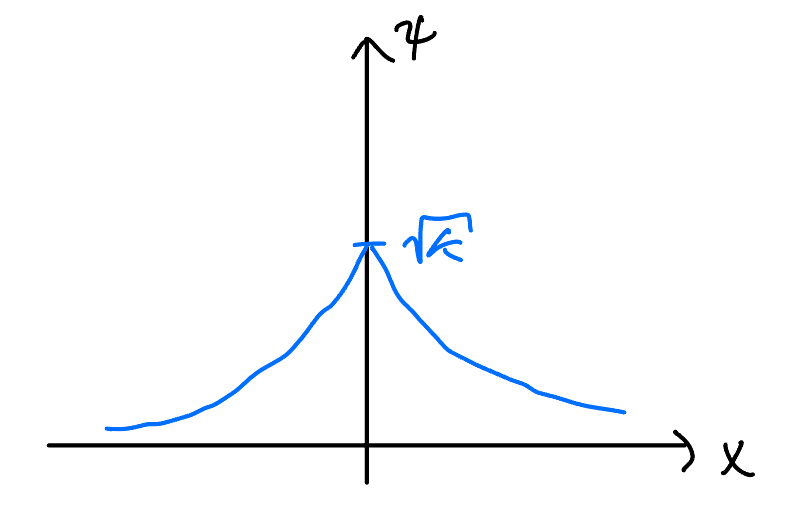
\includegraphics[width=0.5\textwidth]{prob3.jpeg}
   \caption{Sketch of bound state wave function in the potential $V(x) = -V_0 \delta(x)$. Excuse the non-smooth behavior of the sketch, which demonstrates why I did not pursue any career requiring a steady hand!}
   \label{fig:prob3a}
\end{figure}

(b) We now calculate the probability density of the momentum of a function in this potential by taking its Fourier transform:
\begin{eqnarray}
    \begin{aligned}
        \tilde{\psi}(p) &= \sqrt{\kappa} \int_{-\infty}^{\infty} \frac{\dd{x}}{\sqrt{2 \pi \hbar}} e^{-i p x / \hbar} e^{-\kappa |x|} \\
                        &= \sqrt{\frac{\kappa}{2 \pi \hbar}} \Big[ \int_{-\infty}^{0} \dd{x} e^{(\kappa - i p / \hbar) x} + \int_{0}^{\infty} \dd{x} e^{-( \kappa + ip / \hbar ) x} \Big] \\
                        &= \sqrt{\frac{\kappa}{2 \pi \hbar}} \Big[ \frac{1}{\kappa - ip/\hbar} + \frac{1}{\kappa + ip/\hbar} \Big] = \sqrt{\frac{2 \kappa}{\pi \hbar}} ~ \frac{\kappa}{\kappa^2 + (p / \hbar)^2}
    .\end{aligned}
\end{eqnarray}
The probability to find the particle with momentum in the interval $[p,p+\dd{p}]$ is then given as
\begin{eqnarray}
    \tilde{\rho}(p) = |\tilde{\psi}(p)|^2 = \frac{2}{\pi \hbar} \frac{\kappa^3}{[\kappa^2 + (p/\hbar)^2]^2} = \frac{2}{\pi \hbar \kappa} \frac{1}{[1 + (p/\kappa \hbar)^2]^2}
.\end{eqnarray}
Observe that the maximum of this probability density is peaked at $p = 0$ with a value of $2/(\pi \hbar \kappa)$.

From the form of the momentum-space wavefunction, we can also estimate that $\Delta p \sim \hbar \sqrt{\kappa}$\footnote{Again, this comes from the fact that $\Delta p = \sqrt{\expval{p^2}} = \sqrt{\hbar^2 \kappa [ (2/\pi)\int_{-\infty}^{\infty} u^2/(1 + u^2)^2 \dd{u} ]}$}.
Hence, we have $\eqbox{ \Delta x \Delta p \sim \hbar }$.

}


\prob{4 -- Chapter 4 \# 5}{

Consider a particle in the one-dimensional potential $V(x)$, such that $V(x) = \infty$ for $x < 0$ and
\begin{eqnarray}
   V(x) = - V_0 \, \delta(x-a) ~{\rm for}~ x > 0
\end{eqnarray}
where $V_0 > 0$.
Determine whether this potential admits any bound states.

}

\sol{

This potential does have the ability to admit bound states since $\min_{x \in \reals} V(x) = -\infty$.
For $E < 0$, the wave function would be of the form
\begin{eqnarray}
   \psi(x) = 
   \begin{cases}
       0 & x < 0 \\
       A e^{\kappa x} + B e^{-\kappa x} & 0 < x < a \\
       C e^{-\kappa x} & x > a
   ,\end{cases}
\end{eqnarray}
where $\kappa^2 = 2m|E|/\hbar^2$.
Note that we have used the fact that $\psi \rightarrow 0$ as $x \rightarrow \infty$ to rule out the solution $e^{\kappa x}$ in the region $x > a$.

The following boundary conditions must be respected:
\begin{align}
    \psi(0) &= 0 \\
    \psi(a^{-}) &= \psi(a^{+}) \\
    \psi'(a^{+}) - \psi'(a^{-}) &= -\frac{2 m V_0}{\hbar^2} \psi(a)
.\end{align}
Translating this into an statement in terms of $A,~B,~C,~{\rm and}~\kappa$, we have
\begin{align}
    \label{eq:prob4-a}
    A + B &= 0 \\
    \label{eq:prob4-b}
    Ae^{\kappa a} + B e^{-\kappa a} &= Ce^{-\kappa a} \\
    \label{eq:prob4-c}
    - C e^{- \kappa a} - (Ae^{\kappa a} - B e^{-\kappa a}) &= - \frac{v_0}{\kappa} Ce^{-\kappa a}
,\end{align}
where we have defined $v_0 = 2m V_0/\hbar^2$.
Remember that we also have the normalization condition, which imposes an additional constraint on these constants.
Thus, for a non-trivial solution $\{ A,B,C \} $, \erefs{prob4-a}{prob4-c} must be linearly dependent.
\begin{gather}
   \begin{vmatrix}
       \sinh{\kappa a} & -e^{-\kappa a} \\
       \cosh{\kappa a} & (1 - v_0/\kappa) e^{- \kappa a}
   \end{vmatrix}
   = e^{-\kappa a} [ (1 + v_0/\kappa) \sinh{\kappa a} + \cosh{\kappa a} ] = 0 \\
   \tanh{\kappa a} = - \frac{1}{1 - v_0/\kappa} = \frac{1}{v_0/\kappa - 1}
,\end{gather}
where we have used $B = -A$ to reduce the dimensionality (and therefore some complexity) of the problem.
Also note that we have redefined $2A \rightarrow A$.

This is a transcendental equation for $\kappa$, so we cannot solve it directly, but notice that $\kappa a > 0$.
Thus, $\tanh{\kappa a} > 0$, meaning that this equation may only has a solution if $v_0/\kappa > 1$, and hence, a bound state only under this condition.
Additionally, $\tanh{\kappa a} < 1$ for all $\kappa a$.
We thus have a second condition on $v_0/\kappa$:
\begin{eqnarray}
    \frac{v_0}{\kappa} < 2
,\end{eqnarray}
and therefore, generally a bound state exists if and only if
\begin{eqnarray}
    \eqbox{ 1 < \frac{v_0}{\kappa} = \frac{V_0}{E} < 2 \Leftrightarrow \frac{V_0}{2} < E < V_0 }
.\end{eqnarray}

{

\color{red} The above analysis is not entirely correct.
We can rewrite Eq. (43) to read
\begin{eqnarray}
    \tanh{z} = \frac{z}{z_0 - z}
,\end{eqnarray}
where $z = \kappa a$ and $z_0 = v_0 a$.
In this case then, we have something like $f(z) = g(z)$.
Clearly then, whether there is a solution depends on the value of $z_0$.

Let us observe the following:
\begin{enumerate}
    \item $z > 0$ (since $\kappa,a > 0$)
    \item $0 < \tanh{z} < 1$
    \item $z/(z_0 - z) > 0$ for $z \in [0,z_0)$
    \item for $z \in [0,z_0)$, the function $z/(z_0-z)$ is monotonically increasing
    \item $\tanh{0} = 0$ and $0/(z_0-0) = 0$
\end{enumerate}

Clearly, these functions always intersect at $E = 0$, but this is not interesting for this problem since $\psi$ is not normalizable then and hence not a bound state.
We can, however, state whether or not the transcendental equation has a solution (only one if any!).
Since $z/(z_0-z)$ is monotonically increasing, for a bound state to exist, we must have
\begin{eqnarray}
    \dv{z} \tanh{z}|_{z = 0} > \dv{z} \frac{z}{z_0 - z} |_{z=0} \Rightarrow z_0 > 1
.\end{eqnarray}
If this condition is met, though, we must resort to some numerical scheme to determine the energy of the bound state.

}


}

\end{document}
